% 03-results-and-discussions.tex

% Section Title
\section{RESULTS AND DISCUSSIONS} \label{sec:results}

    \subsection{Baseline Performance: Static vs.\ Dynamic}
    
        \subsubsection{Static Case: Monte dei Cappuccini}
        
            The static scenario demonstrated stable GNSS performance. 
            Pseudorange values remained consistent with expected GPS satellite distances (around $2\times10^7$ m). 
            Position estimates clustered within an 8 m radius of the median, and horizontal speed remained near zero, confirming the device was stationary (Figure~\ref{fig:static_pos}). 
            C/No values showed minor fluctuations (Figure~\ref{fig:static_cno}), with a few satellites (e.g., SV 27) experiencing temporary signal degradation. 
            HDOP remained generally low, indicating good satellite geometry. 
            Clock bias increased linearly over time (Figure~\ref{fig:static_wls}), suggesting typical thermal-induced drift.

            \begin{figure}[h!]
                \centering
                \begin{subfigure}{0.23\textwidth}
                    \centering
                    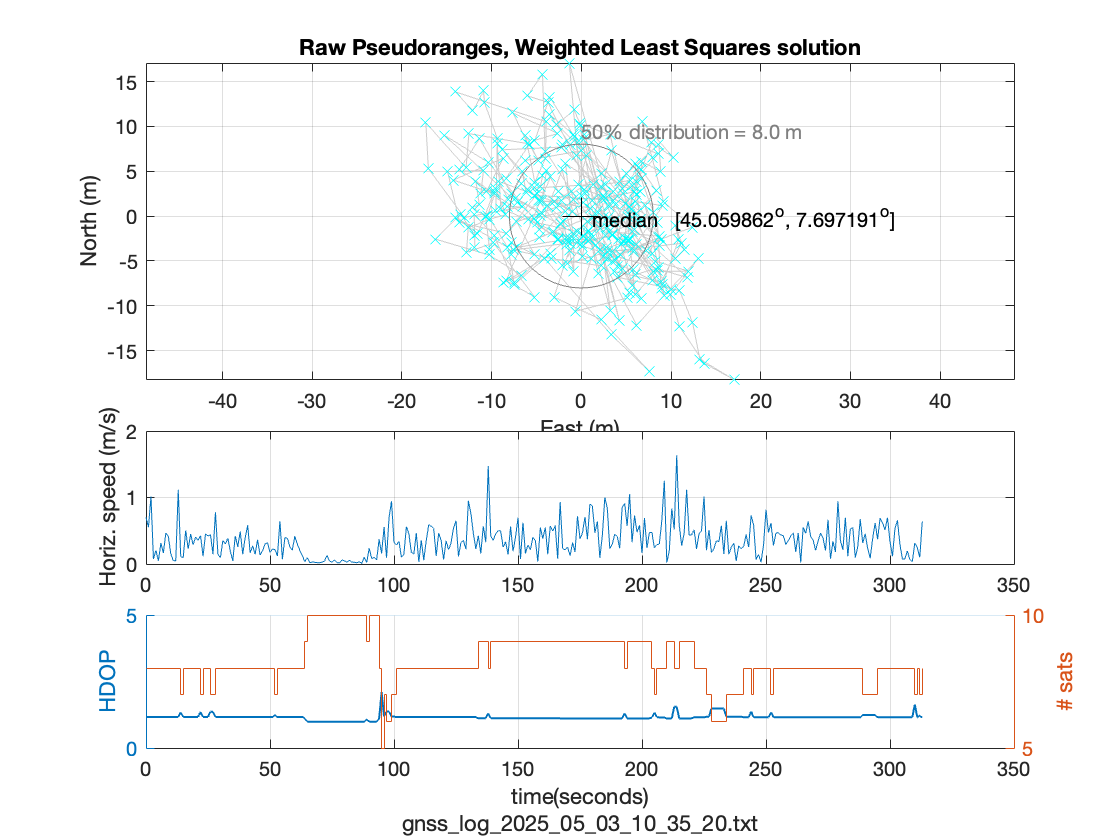
\includegraphics[width=\textwidth]{images/Monte_Cappuccini/filtered/Samsung_A51_Monte_Cappuccini_fig4.png}
                    \caption{Static scenario: Position estimates, horizontal speed, HDOP.}
                    \label{fig:static_pos}
                \end{subfigure}
                \hfill
                \begin{subfigure}{0.23\textwidth}
                    \centering
                    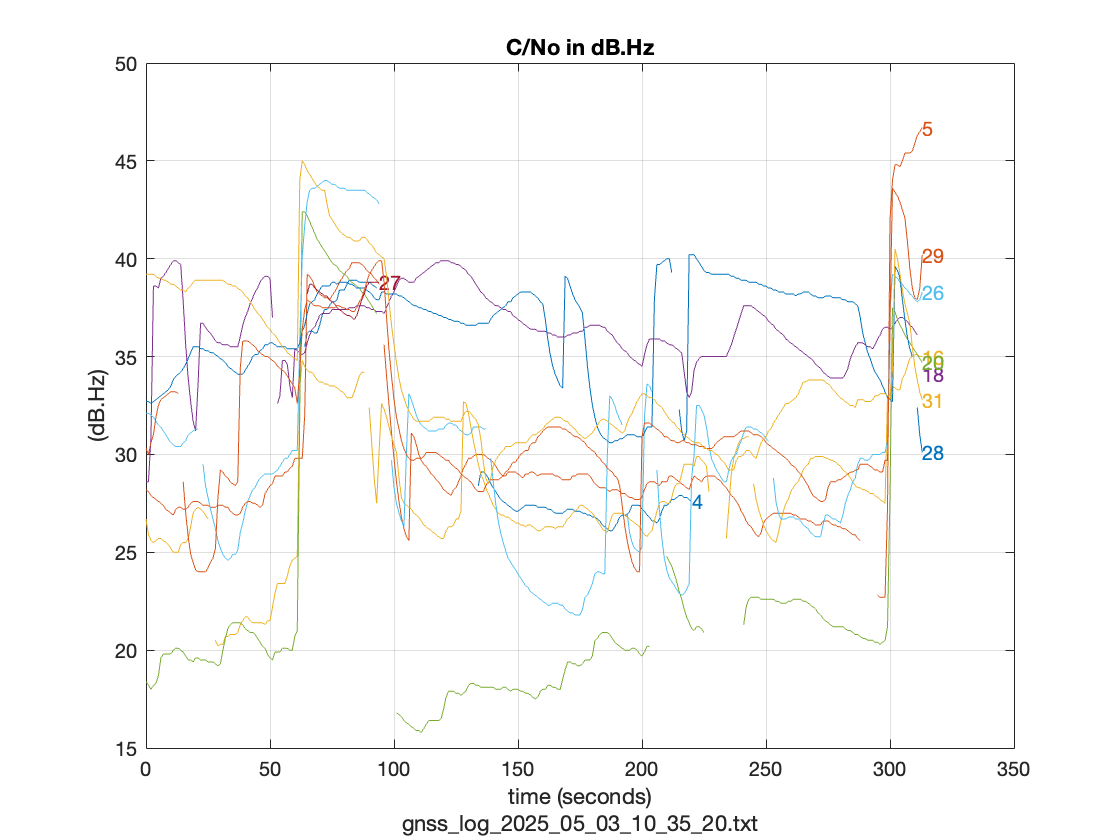
\includegraphics[width=\textwidth]{images/Monte_Cappuccini/filtered/Samsung_A51_Monte_Cappuccini_fig3.png}
                    \caption{Static scenario: Carrier-to-noise ratio over time.}
                    \label{fig:static_cno}
                \end{subfigure}
                \vspace{0.35cm}
                \label{fig:gnss_comparison}
            \end{figure}

            \begin{figure}[h!]
            \centering
            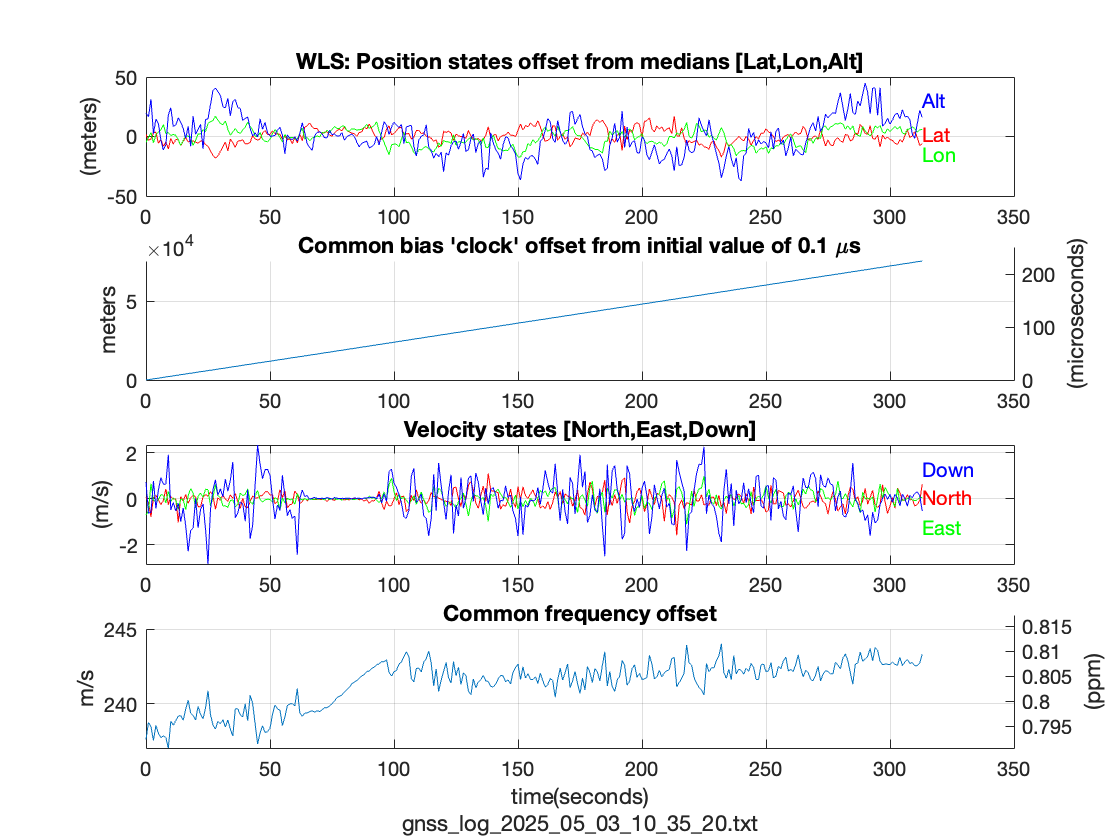
\includegraphics[width=0.23\textwidth]{images/Monte_Cappuccini/filtered/Samsung_A51_Monte_Cappuccini_fig5.png}
            \caption{Static scenario: WLS state offsets and clock bias trends.}
            \label{fig:static_wls}
            \end{figure}

        \subsubsection{Dynamic Case: Tram Ride}
        
            The dynamic scenario exhibited greater measurement variability. 
            Pseudoranges changed more rapidly (Figure~\ref{fig:dynamic_pr}), reflecting motion relative to the satellites. 
            Position estimates were more dispersed, with northward velocity peaking near 20 m/s (Figure~\ref{fig:dynamic_pos}). 
            C/No values fluctuated significantly due to urban obstructions (Figure~\ref{fig:dynamic_cno}), and some satellites showed weak or intermittent signals (e.g., SV 18). 
            HDOP remained within acceptable bounds, although the number of tracked satellites varied. 
            Clock bias again increased linearly but was more affected by motion-induced dynamics (Figure~\ref{fig:dynamic_wls}).

            \begin{figure}[h!]
                \centering
                \begin{subfigure}{0.23\textwidth}
                    \centering
                    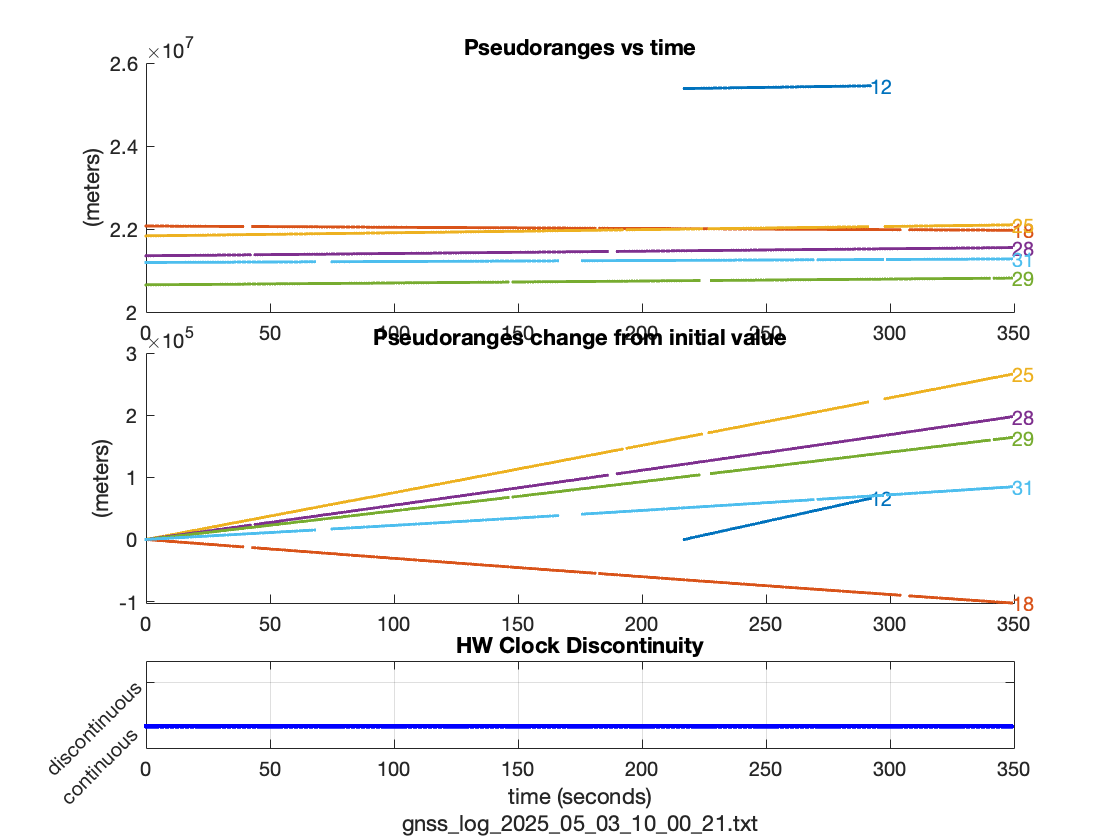
\includegraphics[width=\textwidth]{images/Tram_15_trip_Castello_to_Pescatore/filtered/Samsung_A51_Tram_15_trip_Castello_to_Pescatore_fig1.png}
                    \caption{Dynamic scenario: Pseudoranges and variation over time.}
                    \label{fig:dynamic_pr}
                \end{subfigure}
                \hfill
                \begin{subfigure}{0.23\textwidth}
                    \centering
                    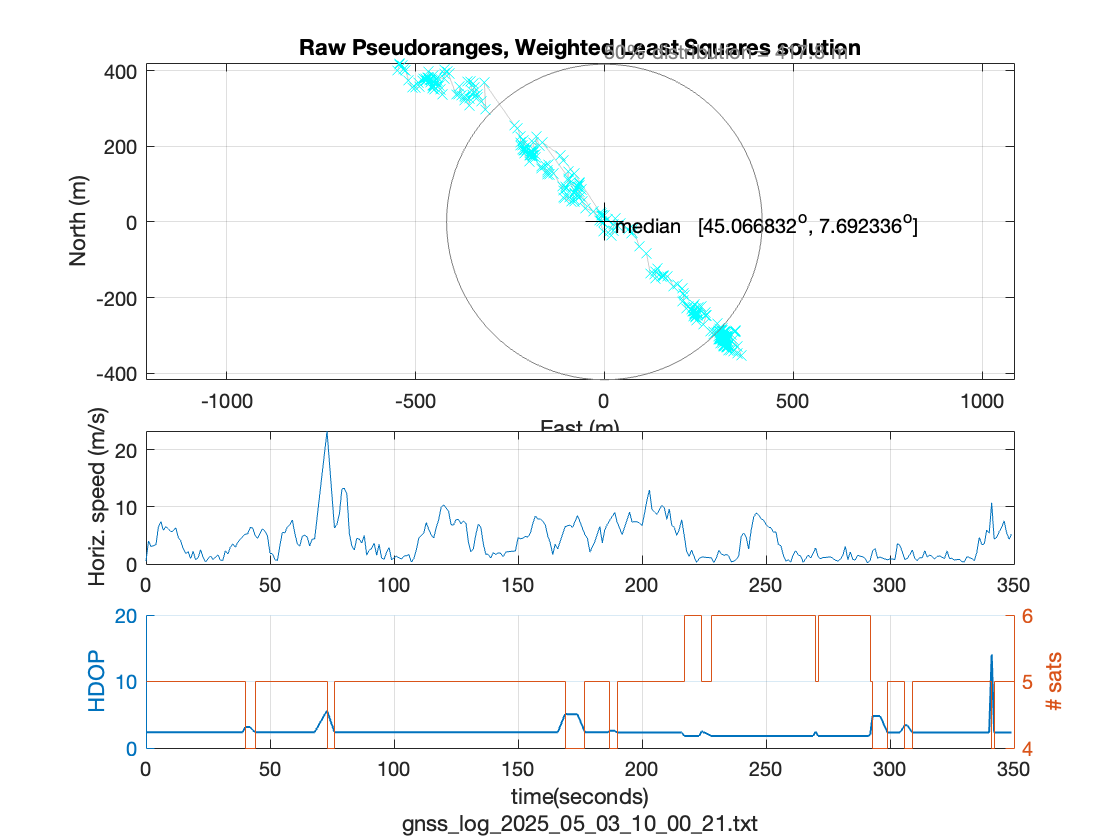
\includegraphics[width=\textwidth]{images/Tram_15_trip_Castello_to_Pescatore/filtered/Samsung_A51_Tram_15_trip_Castello_to_Pescatore_fig4.png}
                    \caption{Dynamic scenario: Position estimates, speed, and HDOP.}
                    \label{fig:dynamic_pos}
                \end{subfigure}
                \vspace{0.35cm}
                \label{fig:gnss_comparison}
            \end{figure}

        
            \begin{figure}[h!]
            \centering
            \begin{subfigure}{0.23\textwidth}
                \centering
                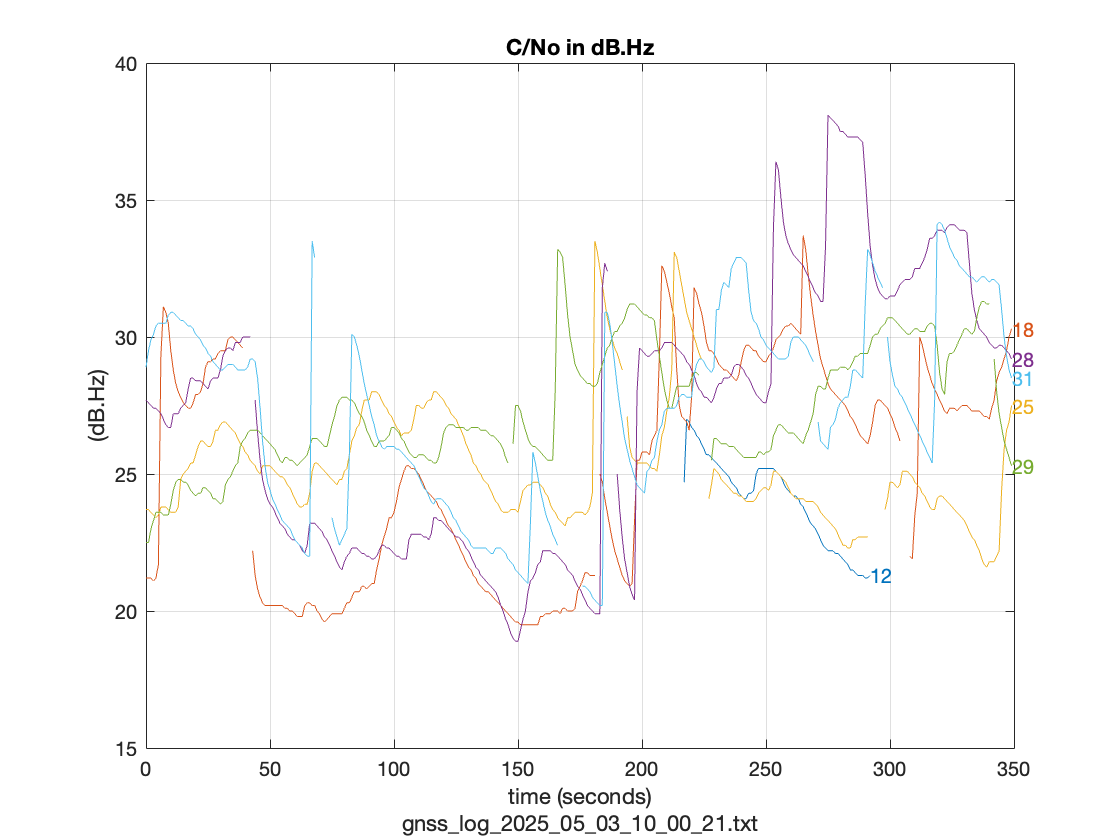
\includegraphics[width=\textwidth]{images/Tram_15_trip_Castello_to_Pescatore/filtered/Samsung_A51_Tram_15_trip_Castello_to_Pescatore_fig3.png}
                \caption{Dynamic scenario: Signal quality (C/No) per satellite.}
                \label{fig:dynamic_cno}
            \end{subfigure}
            \hfill
            \begin{subfigure}{0.23\textwidth}
                \centering
                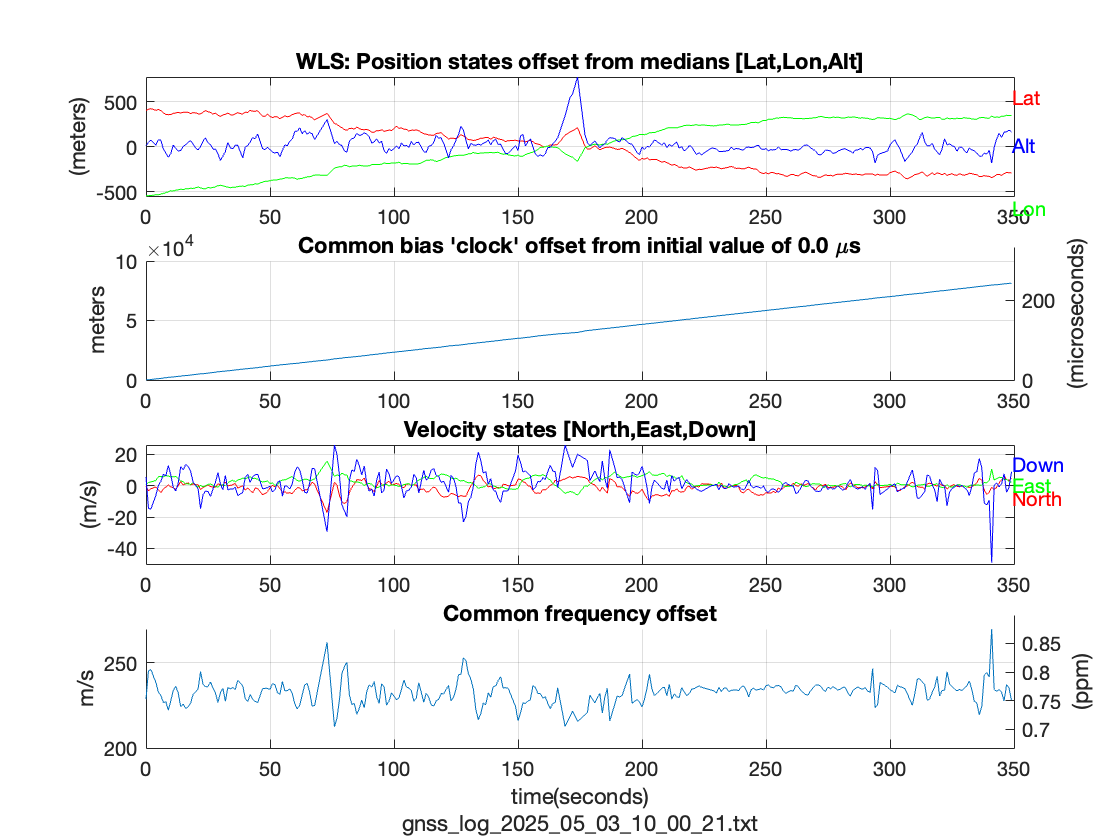
\includegraphics[width=\textwidth]{images/Tram_15_trip_Castello_to_Pescatore/filtered/Samsung_A51_Tram_15_trip_Castello_to_Pescatore_fig5.png}
                \caption{Dynamic scenario: WLS offset and velocity states.}
                \label{fig:dynamic_wls}
            \end{subfigure}
            \vspace{0.35cm}
            \label{fig:gnss_comparison}
            \end{figure}

        \subsubsection{Comparison of Static and Dynamic Performance}
        
            Key differences emerged when comparing static and dynamic scenarios:
            
            \begin{itemize}
                \item \textbf{Pseudorange Trends:} Static measurements showed flat and stable pseudorange lines with minor steps due to satellite handovers or clock corrections (Figure~\ref{fig:static_pr}). In contrast, dynamic measurements exhibited sloped lines, reflecting relative motion to satellites.
                \item \textbf{Doppler Residuals:} In the static case, calculated and reported pseudorange rates aligned closely (Figure~\ref{fig:static_prr}). The dynamic case introduced more noise and discrepancies (Figure~\ref{fig:dynamic_prr}), reflecting movement complexity and potential modeling errors.
                \item \textbf{Signal Quality (C/No):} The static case showed relatively stable C/No values, while the dynamic case had significant fluctuations and lower mean values due to urban interference and multipath effects.
                \item \textbf{HDOP and Satellite Geometry:} HDOP remained low and stable in the static case, while it was slightly higher and more variable in the dynamic scenario due to changing satellite visibility.
                \item \textbf{Error Statistics:} The static case achieved tighter clustering (\textasciitilde8 m radius), whereas the dynamic case showed larger offsets, especially in the latitude/longitude axes (up to \textasciitilde500 m).
                \item \textbf{Velocity and Clock Behavior:} The dynamic case revealed dominant northward motion and larger variation in velocity states. Clock bias trends were similar in both scenarios but more affected by noise in the tram ride.
            \end{itemize}
            
            These differences reflect the impact of movement, signal obstruction, and urban dynamics on GNSS performance, confirming that dynamic environments introduce more variability and require more robust estimation strategies.

            \begin{figure}[h!]
                \centering
                \begin{subfigure}{0.23\textwidth}
                    \centering
                    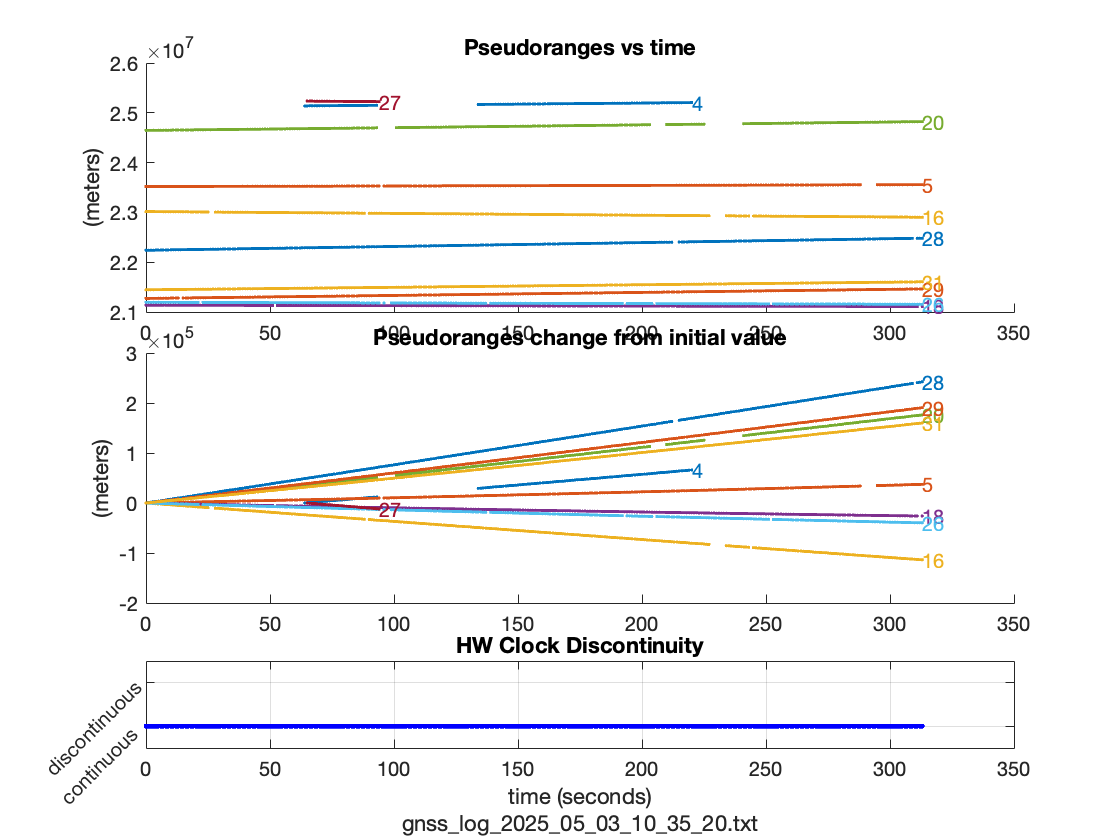
\includegraphics[width=\textwidth]{images/Monte_Cappuccini/filtered/Samsung_A51_Monte_Cappuccini_fig1.png}
                    \caption{Static scenario: Pseudoranges and variation over time.}
                    \label{fig:static_pr}
                \end{subfigure}
                \hfill
                \begin{subfigure}{0.23\textwidth}
                    \centering
                    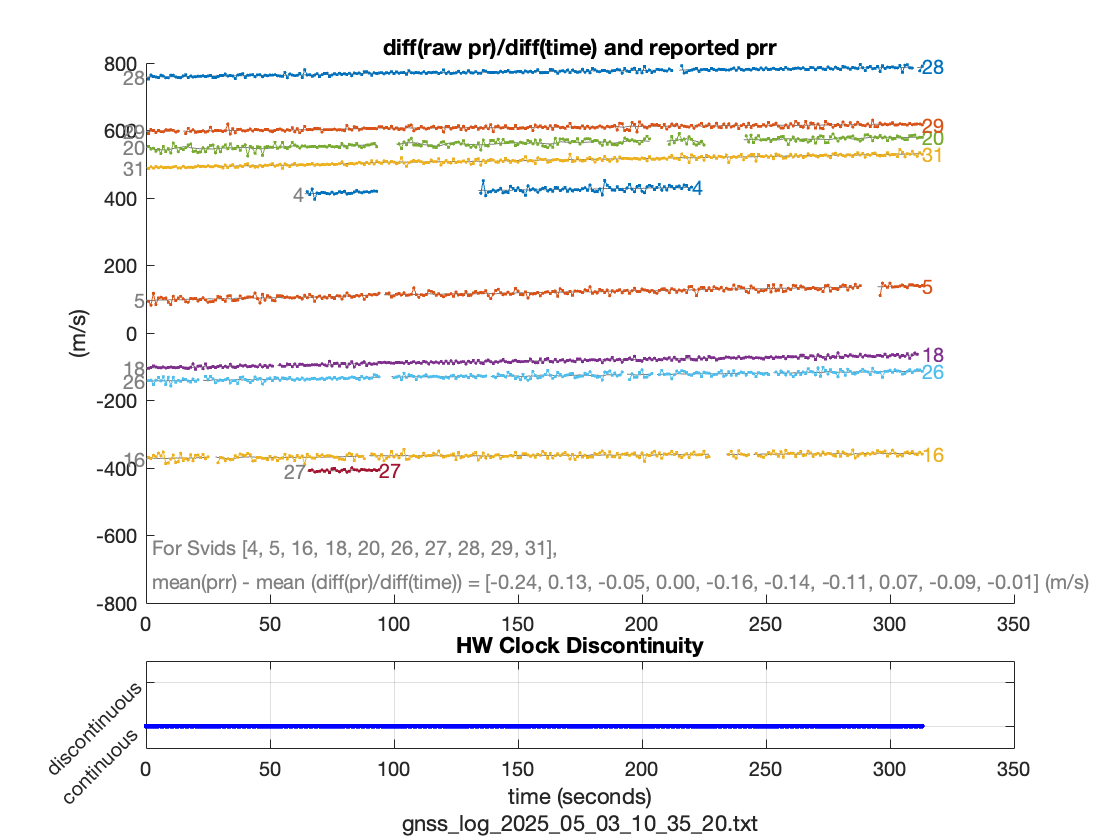
\includegraphics[width=\textwidth]{images/Monte_Cappuccini/filtered/Samsung_A51_Monte_Cappuccini_fig2.png}
                    \caption{Static scenario: Reported vs computed PRR.}
                    \label{fig:static_prr}
                \end{subfigure}
                \vspace{0.35cm}
                \label{fig:gnss_comparison}
            \end{figure}

            \begin{figure}[h!]
            \centering
            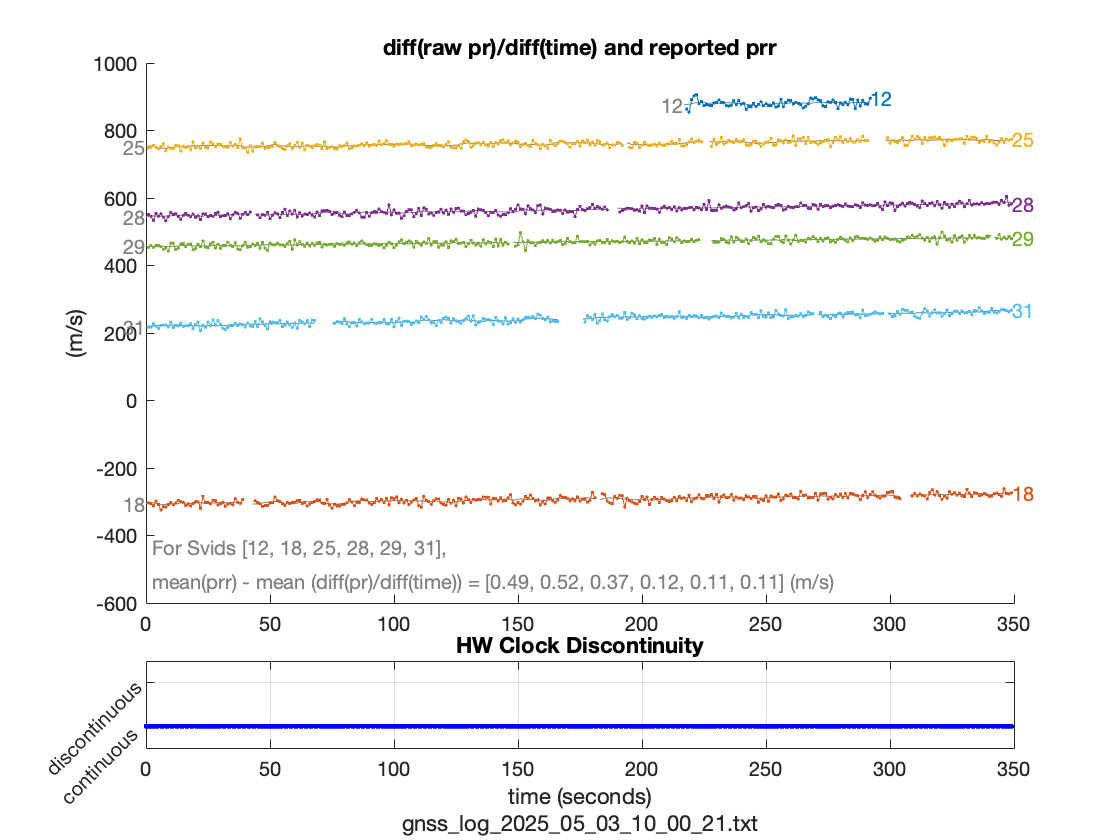
\includegraphics[width=0.23\textwidth]{images/Tram_15_trip_Castello_to_Pescatore/filtered/Samsung_A51_Tram_15_trip_Castello_to_Pescatore_fig2.png}
            \caption{Dynamic scenario: Reported vs computed PRR.}
            \label{fig:dynamic_prr}
            \end{figure}
            
    \subsection{Impact of Spoofed Position}
        
        % Show how the solver output shifts when feeding a false coordinate
        % Note invariance of raw metrics and discuss detection implications

        % content

    \subsection{Effects of Timing Delays}
    
        % Relate applied delays to position and clock-bias anomalies
        % Discuss solver stability and practical consequences

        % content

    \subsection{Interference Effects}
    
        % If performed, explain signal degradations, cycle slips, and accuracy loss

        % content
